\chapter{Dosbarthiad Na\"{i}f Bayes}\label{cha:Dosbarthiad_naif_bayes}
\section{Cefndir}

Mae dosbarthiad na\"{i}f Bayes fel arfer yn cael ei ystyried i fod y dull hawsaf o ddosbarthu sydd ogystal yn weddol gywir. Gall dosbarthiad na\"{i}f Bayes ei ddefnyddio ar ddata di-dor ag arwahanol. I gael creu dosbarthiad ar set ddata di-dor mae rhaid i ni dybio'r fath o ddata sydd gennym, fel arfer y dybiaeth hon yw bod yn dilyn dosraniad normal. O hyn ymlaen fyddwn yn tybio fod y data sydd gennym yn arwahanol. 

Ystyriwch fod gennych set ddata yn cynnwys gwybodaeth am y tywydd am y penwythnosau blaenorol ac p'un ai fod rhyw berson wedi chwarae golff y penwythnos yna. Yn defnyddio'r wybodaeth yma gallwn cyfrifo tebygolrwydd o fynd i chwarae golff rhyw benwythnos i ddod gan ddefnyddio gwybodaeth am y tywydd y benwythnos yna. Enghraifft arall fwy defnyddiol yw categoreiddio dogfenni ar gyfer pwnc, yn syml fydd hyn yn cael ei wneud drwy edrych ar amledd geiriau.\cite{amledd}

\section{Yr Algorithm}

Mae'r dull yma wedi cael ei adeiladu ar sylfaen o reol Bayes sy'n ymwneud gyda thebygolrwydd amodol ag tebygolrwydd ymylol \cite{naif-bayes}. Mae Hafaliad~\ref{eqn:Rheol-Bayes} yn dangos rheol Bayes, lle mae P(A) ydy rhagdebygolrwydd o A, P(A|B) yw'r \^{o}l debygolrwydd o A, ag P(B|A) yw'r tebygolrwydd amodol o B rhoddir A. P(B) yw tebygolrwydd ymylol o B. 

\begin{figure}[H]
\begin{equation}
P(A|B) = \frac{P(A)P(B|A)}{P(B)}
\end{equation}
\label{eqn:Rheol-Bayes}
\end{figure}


Mae'r algorithm yn defnyddio rheol Bayes ag yn ei estyn gan dybio fod pob p\^{a}r o briodoleddau yn dilyn annibyniaeth amodol \cite{scikit-learn-bayes}. Er mwyn gweld hyn wnawn ddiffinio ein newidynnau.

Gadwn i $y$ cynrychioli'r labeli o ddosbarthiadau, hefyd wnawn ddiffinio $x_{i}$ i fod y priodoledd dibynnol lle mae $i \in \{ 1, \dots, n \}$ yn cynrychioli $n$ priodoleddau gwahanol.

Felly mae rheol Bayes yn edrych fel:

\begin{equation}\label{eqn:ol_tebygolrwydd}
P(y|x_{1}, \dots, x_{n}) = \frac{P(y)P(x_{1}, \dots, x_{n}|y)}{P(x_{1}, \dots, x_{n})}
\end{equation}

Yn defnyddio rhagdybiaeth na\"{i}f ar annibyniaeth amodol:

\begin{equation}\label{eqn:tebygolrwydd_amodol}
P(x_{i}|y, x_{1}, \dots, x_{i-1}, x_{i+1}, \dots, x_{n}) = P(x_{i}|y) 
\end{equation}

Gallwn drawsnewid rheol Bayes i reol lawer iawn symlach i'w cyfrifo.

\begin{equation}\label{eqn:rheol_bayes}
P(y|x_{1}, \dots, x_{n}) = \frac{P(y)\Pi^{n}_{i=1} P(x_{i}|y)}{P(x_{1}, \dots, x_{n})}
\end{equation}

Fyddwn yn defnyddio y fformiwla yma i cyfrifo yr \^{o}l tebygolrwydd ar gyfer pob gwerth o $y$ sydd gennym ar gael. Felly oherwydd dim ond $y$ fydd yn newid gennym, gallwn sylwi fod yr enwadur am fod yn hafal i bob cyfrifiad, felly i gymharu yr \^{o}l tebygolrwydd i bob gwerth gallwn ei anwybyddu. Felly i cymharu tebygolrwydd am wahanol labeli fyddwn yn cymharu drwy edrych ar y rhifiadur yn unig.

Mae sut rydym yn cyfrifo $P(x_{i}|y)$ yn dibynnu yn hollol ar y priodoledd, gan ein bod am edrych ar set ddata sy'n gategoreiddiol yn y tiwtorialau fyddwn yn edrych ar ffurf dosbarthiad na\"{i}f Bayes gategoreiddiol yn benodol. Felly i ddata wedi'i chategoreiddio, ar gyfer categori k ag dosbarth h:

\begin{equation}\label{eqn:naif-bayes-categoreiddiol}
P(x_{i} = k|y = h) = \frac{N_{k,h}}{N_{h}}
\end{equation}

Lle mae $N$ yn dynodi'r nifer o samplau. Gan fod y rhif yma o fewn lluoswm ac mae'n bosib cael tebygolrwydd o $0$, fyddem yn defnyddio ffurf llyfnhau Laplace i addasu ein niferoedd i fod yn fwy tebygol i ddosbarthiad unffurf. Mi wnawn wneud hyn gan gyflwyno newidyn newydd $\theta$ a dynodwyd $n_{i}$ y nifer o categoreiddiau gwahanol o fewn priodoledd $i$. Yna:

\begin{equation}\label{eqn:llyfnhau-laplace}
P(x_{i} = k|y = h; \theta) = \frac{N_{k,h} + \theta}{N_{h} + \theta n_{i}}
\end{equation}

Y fwyaf mae'r gwerth o $\theta$, y fwyaf agos i'r dosraniad unffurf fydd y niferoedd yn mynd. Mae'r tebygolrwydd ymylol $P(y)$ yn ddigon hawdd i'w cyfrifo:

\begin{equation}\label{eqn:ymylol}
P(y) = \frac{N_{h}}{N}
\end{equation}

Felly i gloi, gallwn ysgrifennu fformiwla dosbarthiad na\"{i}f Bayes categoreiddiol fel

\begin{equation}\label{eqn:dosbarthiad-categoreiddiol}
P(y|x_{1}, \dots, x_{n}; \theta) = \frac{N_{h}}{N P(x_{1}, \dots, x_{n})} \prod^{n}_{i=1} \frac{N_{k,h} + \theta}{N_{h} + \theta n_{i}} 
\end{equation}

ac felly:

\begin{equation}\label{eqn:naif-bayes-syml}
P(y|x_{1}, \dots, x_{n}; \theta) \propto \frac{N_{h}}{N} \prod^{n}_{i=1} \frac{N_{k,h} + \theta}{N_{h} + \theta n_{i}}
\end{equation}

\section{Tiwtorial yn R}

Ar gyfer y tiwtorial yma fydd rhaid i chi lawrlwytho'r set ddata o \url{https://dysgupeirianyddol.github.io/lawrlwythiadau/}. Mae'r set ddata rydym yn edrych ar yn cynnwys gwybodaeth am $200$ person a wnaeth pleidleisio mewn etholiad. Mae'r data yn cynnwys y blaid wleidyddol a wnaeth phob un pleidleisio am ag y priodoleddau canlynol: gwlad, rhyw, os yw'n hapus gyda'r blaid yn bw\^{e}r, math o d\^{y} ag os yw'n berchen ar fwy nag un t\^{y}.

Unwaith fod y set ddata wedi lawrlwytho, wnawn lwytho'r data i mewn a'i arbed fel newidyn. Dewisom etholiad fel newidyn.

\begin{minted}[bgcolor=green!7]{r}
> etholiad <- read.csv("etholiad.csv")
\end{minted}

Nawr gallwn weld y data gan redeg y canlynol:

\begin{minted}[bgcolor=green!7]{r}
> View(etholiad)
\end{minted}

\begin{figure}[H]
\begin{center}
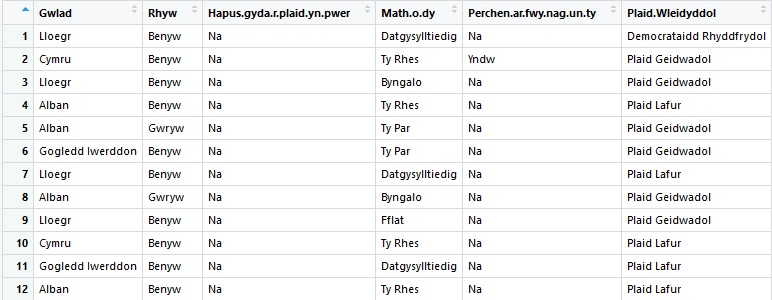
\includegraphics[width=0.8\linewidth]{../img/data_dosbarthiad.jpg}
\label{fig:data_dosbarthiad}
\caption{Data ar etholiad.}
\end{center}
\end{figure}

Mae'r ffwythiant canlynol yn R yn cyfrifo'r tebygolrwydd amodol pryd rydym yn gwybod y blaid, gall y ffwythiant cael ei ddefnyddio ar gyfer unrhyw blaid fel gwelwn yn cael ei ddefnyddio pan fyddem yn rhagfynegi hwyrach ymlaen.

\begin{minted}[bgcolor=green!7]{r}
> tebygolrwydd_amodol <- function(plaid, colofn, gwerth, data)
+ {
+    rhifiadur <- sum(data[which(data[,"Plaid.Wleidyddol"]==plaid),
+                                names(data)[colofn]]==gwerth)+1 
+    enwadur <- length(data[which(data[,"Plaid.Wleidyddol"]==plaid),names(data)[colofn]])
+               +length(levels(etholiad[,colofn])))
+    rhifiadur/enwadur
+ }
\end{minted}

Gwelwn fod y ffwythiant uchod yn defnyddio'r dull cyfrif ffug. Yn y ffwythiant nesaf rydym yn cyfrifo y tebygolrwydd o bob plaid yn unigol.

\begin{minted}[bgcolor=green!7]{r}
> tebygolrwydd <- function(plaid, data)
+ {
+   sum(etholiad[,"Plaid.Wleidyddol"]==plaid)/length(etholiad[,"Plaid.Wleidyddol"])
+ }
\end{minted}

Nawr mae gennym y ddwy gydran o'r fformiwla na\"{i}f Bayes. Mae'r ffwythiant isod yn defnyddio'r ddau ffwythiant blaenorol i gyfrifo'r tebygolrwydd o ddosbarthu y plyg i bob plaid. Wnawn wneud hyn gan creu fector gyda'r tebygolrwydd i bob plaid yn drefn briodol i hyn wnaethom gyda'r fector pleidiau ac yna cyfrifo'r uchafswm.

\begin{minted}[bgcolor=green!7]{r}
> rhagfynegi <- function(data, plyg)
+ {
+   pleidiau <- c("Plaid Geidwadol", "Plaid Lafur", "Democrataidd Rhyddfrydol", "Arall")
+   fector_tebygolrwydd <- c()
+   for (i in pleidiau)
+   {
+     tebygolrwydd_plaid <- 1
+     for (j in 1:(length(names(data))-1))
+     {
+       tebygolrwydd_plaid <- tebygolrwydd_plaid * 
+                             tebygolrwydd_amodol(i, j, plyg[j], data)
+     }
+     tebygolrwydd_plaid <- tebygolrwydd_plaid * tebygolrwydd(i, data)
+     fector_tebygolrwydd <- c(fector_tebygolrwydd, tebygolrwydd_plaid)
+   }
+   return(pleidiau[which.max(fector_tebygolrwydd)])
+ }
\end{minted}

Nawr wnawn greu plyg i gael dosbarthu ei blaid. Defnyddiwn y nodweddion yma:

\begin{minted}[bgcolor=green!7]{r}
> plyg <- c("Lloegr", "Benyw", "Na", "Ty Rhes", "Na")
\end{minted}

\begin{minted}[bgcolor=green!7]{r}
> rhagfynegi(data = etholiad,plyg = plyg)
[1] "Plaid Lafur"
\end{minted}

Defnyddiwn y ffwythiant a chawsom allbwn fod y plyg yn cael ei dosbarthu i bleidleisio am Lafur. Wnawn creu plyg arall i profi'r algorithm:

\begin{minted}[bgcolor=green!7]{r}
> plyg <- c("Lloegr", "Gwryw", "Yndw", "Ty Rhes", "Yndw")
\end{minted}

\begin{minted}[bgcolor=green!7]{r}
> rhagfynegi(data = etholiad,plyg = plyg)
[1] "Plaid Ceidwadol"
\end{minted}

Gan ddefnyddio'r ffwythiant cafodd y plyg yma ei dosbarthu i bleidleisio am Blaid Geidwadol.

\section{Tiwtorial yn Python}

Yn y tiwtorial hwn fyddwn yn defnyddio set ddata o ryw etholiad sydd yn cynnwys y priodoleddau o $200$ berson, y priodoleddau yw gwlad breswyl, rhyw, os yw'n hapus gyda'r blaid yn bw\^{e}r, math o d\^{y} sydd gennym ac os oes gennym fwy nag un t\^{y}. Mae'r set ddata ar gael ar y wefan \url{https://dysgupeirianyddol.github.io/lawrlwythiadau/}. I gychwyn dosbarthiad na\"{i}f Bayes yn Python mae rhaid llwytho'r pecyn \mintinline{python}{pandas}. Llwythwn y pecyn fel:

\begin{minted}[bgcolor=cyan!7]{python}
>>> import pandas as pd
\end{minted}

Yna wnawn lwytho'r data. Yna fedrem weld y data gan ddefnyddio \mintinline{python}{data.head()}.

\begin{minted}[bgcolor=cyan!7]{python}
>>> data = pd.read_csv('etholiad.csv')
>>> data.head()
\end{minted}

Gwelwn fod pob priodoledd yn ddata wedi'i chategoreiddio sydd yn gadael ni ddefnyddio 

\begin{figure}[H]
\begin{center}
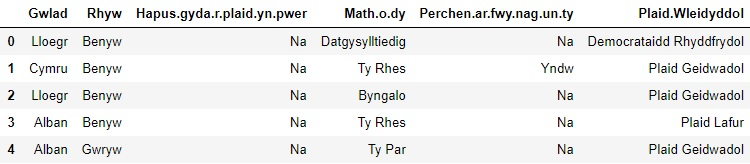
\includegraphics[width=0.8\linewidth]{../img/data_dosbarthiad_python.jpg}
\label{fig:data_dosbarthiad_python}
\caption{Data etholiad yn Python}
\end{center}
\end{figure}

Byddwn yn creu ddau ffwythiant, un i'r ddau debygolrwydd sy'n cael ei chynnwys yn y rhifiadur o'r fformiwla na\"{i}f Bayes. Mae'r ffwythiant cyntaf yn edrych ar y tebygolrwydd amodol, fydd y ffwythiant yn cymryd mewnbwn o blaid, colofn, gwerth y plyg ag y data defnyddiwn. Mae'r ffwythiant hefyd yn defnyddio cyfrif-ffug i wneud yn si\^{w}r fydd yna ddim tebygolrwydd o faint $0$ yn cael ei lluosi yn y lluoswm nes ymlaen.

\begin{minted}[bgcolor=cyan!7]{python}
>>> def tebygolrwydd_amodol(plaid, colofn, gwerth, data):
...     rhifiadur = len(data[(data["Plaid.Wleidyddol"]==plaid)&
...                          (data[colofn]==gwerth)]) + 1
...     enwadur = len(data[data["Plaid.Wleidyddol"]==plaid])+len(data[colofn].unique())
...     return rhifiadur/enwadur
\end{minted}

Ag isod mae gennym y ffwythiant ar gyfer cyfrifo'r tebygolrwydd o ryw blaid. 

\begin{minted}[bgcolor=cyan!7]{python}
>>> def tebygolrwydd(plaid, data):
...     return len(data[data["Plaid.Wleidyddol"]==plaid]) / len(data)
\end{minted}

Yna i greu rhif pendant ar gyfer y rhifiadur o'r tebygolrwydd o bob plaid ac i ddewis yr uchafswm.

\begin{minted}[bgcolor=cyan!7]{python}
>>> def rhagfynegi(data, plyg):
...     colofnau = data.columns[:-1]
...     pleidiau = data['Plaid.Wleidyddol'].unique()
...     tebygolrwyddau = {p: 1 for p in pleidiau}
...     for plaid in pleidiau:
...         for i, colofn in enumerate(colofnau):
...             gwerth = plyg[i]
...             tebygolrwyddau[plaid] *= tebygolrwydd_amodol(plaid, colofn, gwerth, data)
...         tebygolrwyddau[plaid] *= tebygolrwydd(plaid, data)
...     return max(tebygolrwyddau.keys(), key=lambda x: tebygolrwyddau[x])
\end{minted}

Dyma'r plyg fyddem yn defnyddio i drio rhagfynegi ei blaid drwy ddosbarthu. 

\begin{minted}[bgcolor=cyan!7]{python}
>>> plyg = ["Lloegr", "Benyw", "Na", "Ty Rhes", "Na"]
\end{minted}

Gawn ni allbwn o blaid lafur o redeg y ffwythiant \mintinline{python}{rhagfynegi} ar ein plyg.

\begin{minted}[bgcolor=cyan!7]{python}
>>> rhagfynegi(data, plyg)
'Plaid Lafur'
\end{minted}

Nawr wnawn drio plyg wahanol i'r algorithm drio rhagfynegi ei blaid.

\begin{minted}[bgcolor=cyan!7]{python}
>>> plyg = ["Lloegr", "Gwryw", "Yndw", "Ty Rhes", "Yndw"]
\end{minted}

\begin{minted}[bgcolor=cyan!7]{python}
>>> rhagfynegi(data, plyg)
'Plaid Geidwadol'
\end{minted}

Gwelwn drwy ddefnyddio'r algorithm ar blyg gwahanol cafodd ei ddosbarthu i Blaid Geidwadol.